\documentclass[11pt]{ujarticle}\sloppy
\usepackage{funinfosys}
\usepackage[hyphens]{url}
\usepackage[dvipdfmx]{graphicx}
\author{% 
b1021204 西侑亮\\指導教員 : 松原克弥
}		
\course{Information Systems Course}

\title{独自管理インターフェースを持つ未来大クラウドシステムのIaC対応}
\etitle{FUN Cloud System Which Have Unique Management Interface
\\Implementatios of IaC}
\eauthor{Yusuke Nishi}
\abstract{大学のプログラミングや情報科学の講義において,実践的な技能を習得することを目指し,繰り返し演習が行われている.今日では,演習のための統一環境を用意するためにクラウドシステムによる仮想マシンを用いる.しかし,仮想マシンの作成や設定を学生人数分用意するためには多くの手順を必要とすることが課題である.
クラウドシステムをコードで管理する手法であるInfrastructure as Code(IaC)を用いることで効率的に管理することが期待できる.
本研究では,公立はこだて未来大学にて使用されているクラウドシステムを,IaCに対応させることにより,効率よく統一環境を用意し,講義の効率化を目指す.
}
\keywords{Cloud System, IaC, 公立はこだて未来大学}
\eabstract{
	In lecture programming or Information Systems, give a seminar on Information Processing.
	Nowadays, virtual machines based on cloud systems are used to prepare a unified development environment for the seminar. However, the problem is that many processes are needed to create and configure virtual machines for the number of students. Using of Infrastructure as code (IaC) that the approach of managing Cloud systems by code can be expected to manage efficiently.The study's goal is to improve seminar efficiency by efficiently constructing a unified development environment for the cloud system used at Future University Hakodate (FUN) that is compatible with IaC.
	}

\ekeywords{Cloud System, IaC, Future University of Hakodate}
\begin{document}
\maketitle


\section{背景と目的}
\label{sec:intro}
近年,公立はこだて未来大学をはじめとする教育機関での,情報科学の演習講義において,教室にPCを設置し統一された演習環境を用意する授業スタイルから,
学生個人のPCを用いて学習するBYOD(Bring Your Own Device)が加速度的に浸透している.BYODにおいて学生が購入するPCの環境はOSや内部設定が異なる場合が多い.
そのため,公立はこだて未来大学(以降,未来大)や大阪大学をはじめとする大学は,クラウドシステムを利用して仮装マシンを学生に提供することにより統一された演習環境を用意している[1].

クラウドシステムを利用した情報科学の演習講義の事例が増加するとともに,新たな課題も浮上している.
例えば,仮想マシンの設定を行うにあたり授業時間や教員の手間が必要となることである.
未来大における,情報科学の演習講義の一つである並列分散処理において,複数台の仮想マシンを用意して一つのプログラムを並列分散実行する演習がある.
2023年度に行われた同科目では未来大クラウドシステムでの実行方法やマシンの初期設定について合計10ページにわたる解説が行われている.
講義を受講している学生分の仮想マシンを初期設定を済ませてから学生に配布することができれば授業の効率向上を見込める.

%目的

本研究は,クラウドシステムを利用する情報科学の演習講義における効率化を目指し,演習用クラウドシステムのInfrastructure as Code(以降,IaC)対応について対応・評価を行う.
IaCとは,プログラミング言語で書かれたコードを実行することによりITインフラストラクチャを作成管理する手法のことを意味する[2].
Micheleら[3]は,IaCにを用いることで,仮想環境構築の再現性,再利用性,効率性で多くの利点をもたらすことが述べられいる.



\section{Terraform}

本研究では,IaCフレームワークの一つであるTerraformをもちいる.数多あるIaCフレームワークの中からTerraformを選んだ理由として,
デファクトスタンダードである,つまり利用者がもっとも多く,対応するクラウドプロバイダが多いからである.
TerraformはAmazon Web Services(以降,AWS)や
Microsoft Azure,Google Cloud Platformなどのクラウドプロバイダに対応していて,Terraformのコードを学習することで他のプロバイダーを操作する時に同様の操作で管理することができる.
チュートリアルも手厚く公開されており学習が容易である.さらに,Terraform Custom Framework Providerが公開されており,新規のプロバイダーのIaC対応化のための情報が公開さている.
作成したカスタムフレームワークはTerraformを介して,世界中に公開することも可能である.


\begin{figure}[h]
	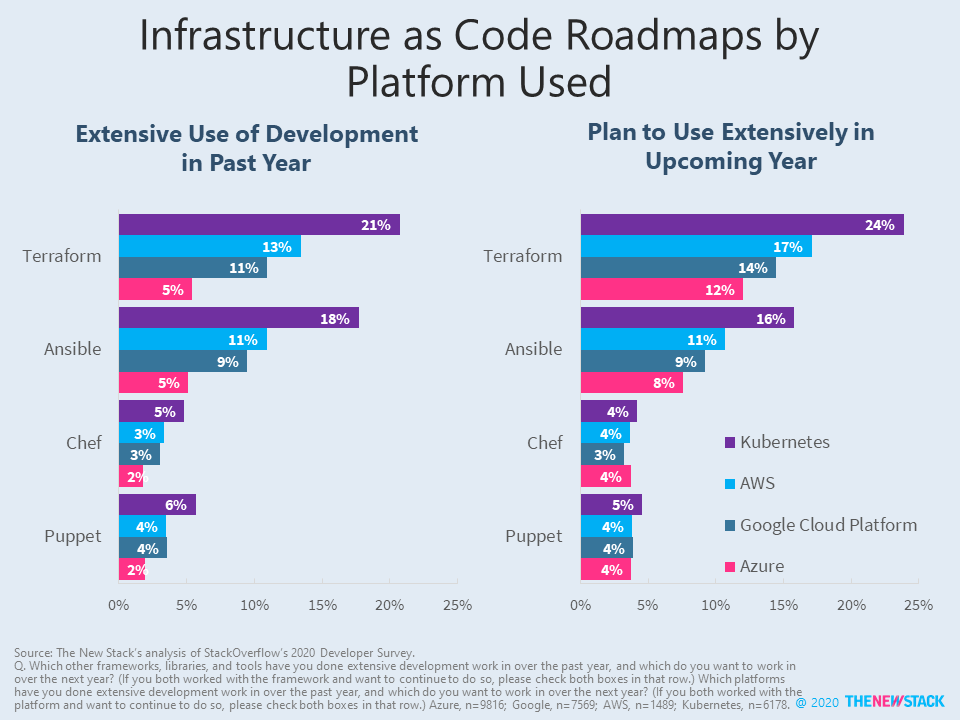
\includegraphics[width=1\linewidth]{./images/terraform.png}
	\caption{2020年のIaCプラットフォームの利用率比較[4]}
  \label{fig:terraform}
\end{figure}


また,プロビジョニング機能を備えている点も理由に挙げる.プロビジョニング機能とは仮装マシンの作成・起動時にデータベース,キャッシュ,ロードバランサ,キュー,サブネットの設定,ルーティングのルールの設定を行う機能である.
Terraformでは仮想マシン作成・起動後にマシンに対してSSH接続を行いプロビジョニング機能を実現している.これらの機能を用いることにより,マシン設定を記述したコードを学生に配布し,実行させることで容易かつ効率的な演習に用いる統一環境環境の準備が可能になると期待する.

\section{提案}


本研究は,未来大クラウドシステムをIaC対応化させることを提案する.これにより,仮想マシンをコードで管理することが可能となり,コードの配布で統一環境構築が可能となり,
従来の演習準備と比べ,大幅な時間短縮を期待できる.


\section{実装}

本提案の実装では,Terraform Custom Framework Providerを用いて未来大クラウドシステムを操作して仮想マシンを管理する.
クラウドシステムを操作するためには,管理に用いるApplication Programming Interface(以降,API)が公開されている必要がある.
しかし,未来大クラウドシステムではAPIが公開されていない.公開されていない理由として以下の理由が挙げることができる.
未来大クラウドシステムでは,学生がアカウント認証をして,学生それぞれが別々の仮想マシン管理画面(WebAPI)へと遷移する.その後,マシン作成や起動,削除を行う.
一見,学生それぞれが独立してクラウドシステムを管理しているように見えるが,内部では学生それぞれの管理要求を集約し,一つのAWSアカウントが管理している.
そのため,学生のアカウントに対して個別にAPIを公開するためには,システムの大幅な改変が不可欠であり,多くの労力と費用を要する.


\begin{figure}[h]
	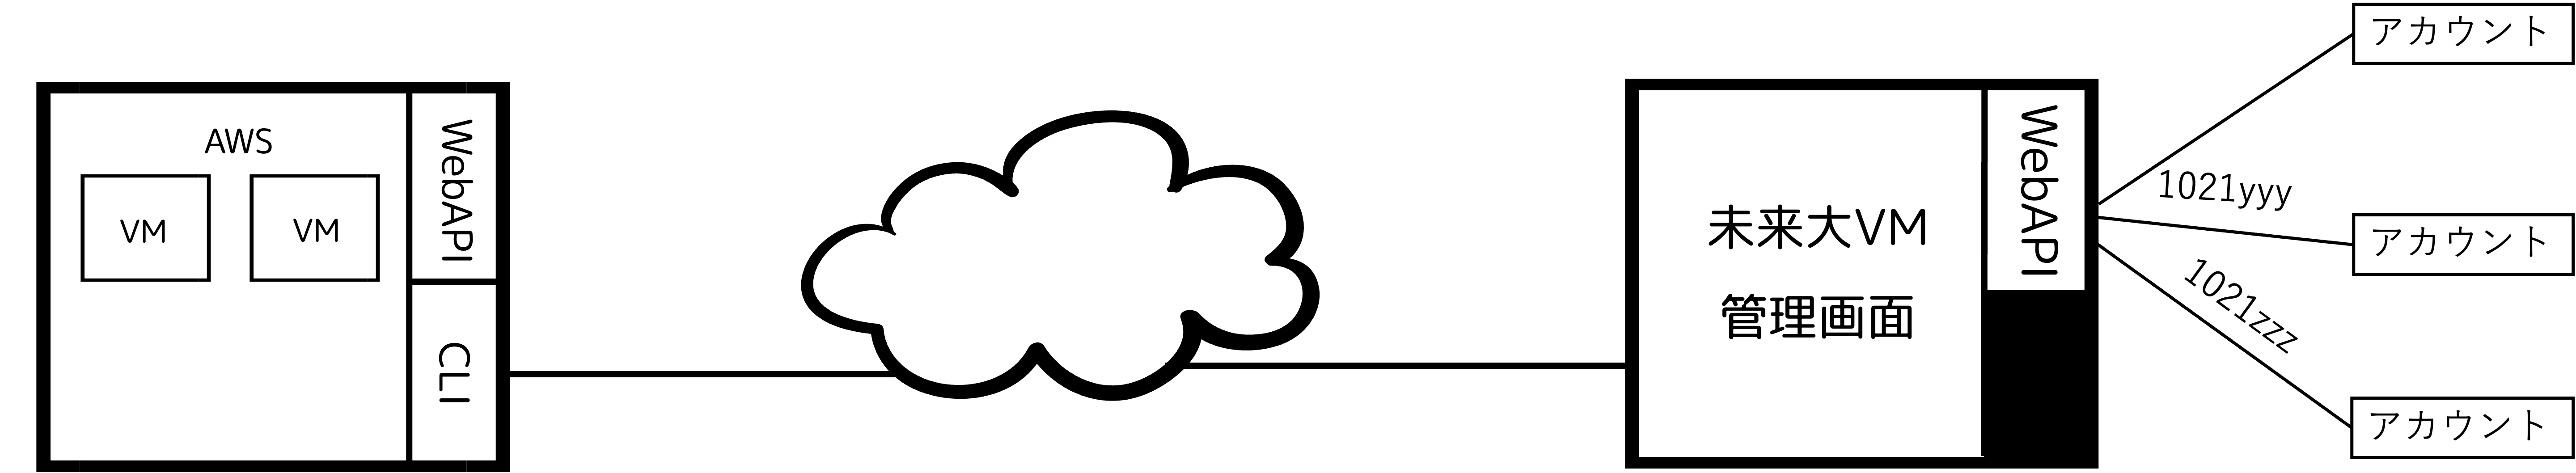
\includegraphics[width=1\linewidth,height=2cm]{./images/cloud.png}
	\caption{未来大クラウドシステムの構造}
  \label{fig:cloud}
\end{figure}

そこで,APIを用いるのではなく,スクレイピングを用いた操作により,クラウドシステムの操作を実現する.
スクレイピングとは,WEBページ上のHTMLやCSSに存在するタグやデータ構造を解析し.構造化されているデータをプレーンなデータへと抽出し変換する技術である.
し変換する技術である.スクレイピングはプログラムを使用して行われ,目的のWeb ページのHTMLデータを解析し,特定の情報をユーザからのリクエストに応じて自動的に取り出すことを可能にする.
スクレイピングは,データ解析,機械学習,市場調査,自動化テスト,自動入力など,多様な分野で使用されており,データ収集手段として注目を浴びている.
ログイン認証が必要なページや,フォーム入力が必要な場合にも,スクレイピング技術は有効であり,このような場合,ヘッドレスブラウザや専用のライブラリを使用し,自動的にフォームを入力,ログインプロセスを完了させることができる.
スクレイピングを活用し,未来大クラウドシステムのWebAPIを自動で操作することにより,未来大クラウドシステムの操作を実現する.


\begin{figure}[h]
	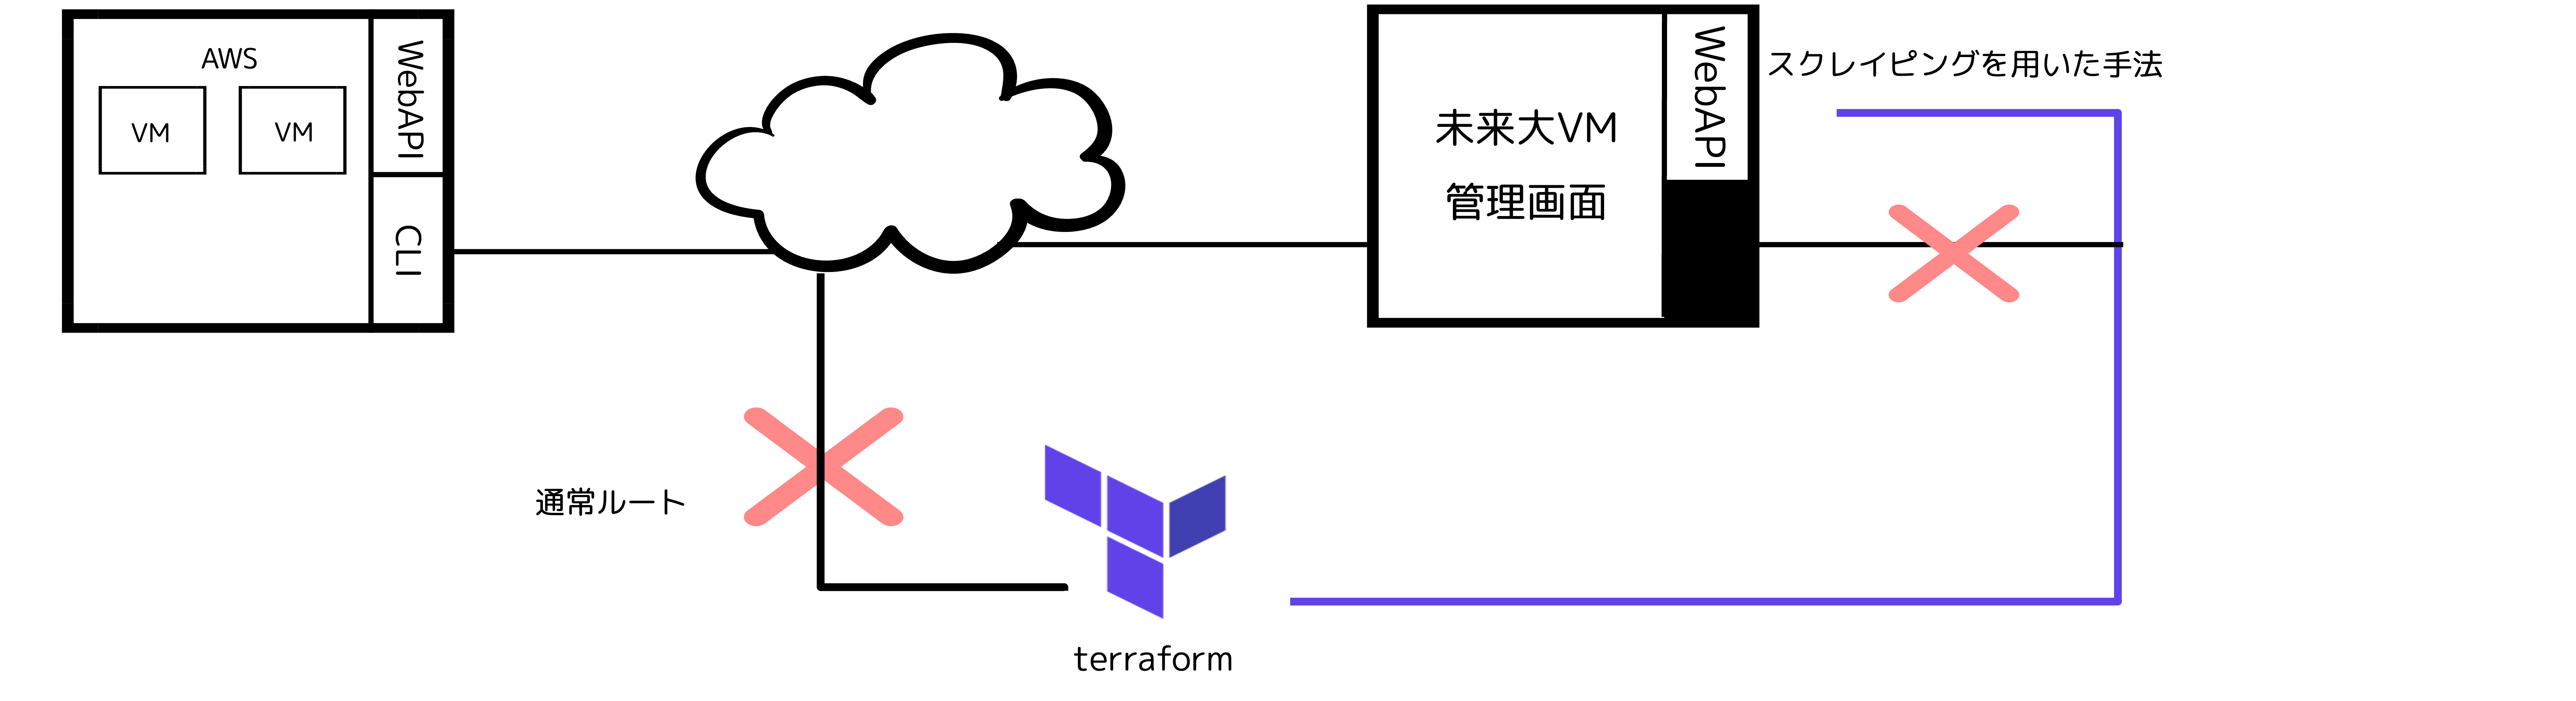
\includegraphics[width=1\linewidth]{./images/scraping.png}
	\caption{スクレイピングによる未来大クラウドシステムの管理}
  \label{fig:scraping}
\end{figure}


Agoutiとは,Web自動化に優れたスクレイピングツールで,ユーザーの動きを再現してブラウザを自動操作することに秀でている.
また,ドロップダウンメニューの選択やボタンクリック,フォームへの自動入力を実行することが容易であり,
ログイン認証への対応の操作に適している.
また,AgoutiはGo言語上で使用可能なツールである.



本研究で操作する未来大クラウドシステムのWebAPIはドロップダウンメニューによる選択やボタンクリックによる画面遷移,ユーザー認証画あり
動的なWebページである.また,Terraform Custom Framework ProviderはGo言語でプログラミングされている.本研究で用いるスクレイピングツールとしてAgoutiを採用した.


Agoutiを動作させるWebDriverとして,ChromeDriverを採用した.WebDriverとは, Web ページへの移動やユーザ入力などが可能なオープンソースフレームワークである.
ChromeDriverはGoogleChromeを自動制御するためのWebDriverである.ChormeDriverはクロスプラットフォーム対応しており,様々なオペレーティングシステム上で動作する.
また,Chromeブラウザの内部APIを直接利用しているため高速で動作する.本研究では,学生が所有するPC環境が異なっていても同様に動作することが望ましい.

未来大クラウドシステムの画面遷移では,最初にユーザ認証画面が存在する.ユーザーが作成したTerraformの仮想マシン設定ファイルの情報(以降,設定ファイル)を元に,スクレイピングを用いてユーザー情報とパスワードを
自動入力し,ボタンクリックを行うことで環境選択画面に遷移する.環境選択では,年度や時期,受講している講義ごとに異なる環境を選択することが可能である.設定ファイルで指定された環境選択をドロップダウンから選択し,仮想マシン管理へ遷移する.
仮想マシン管理画面では,作成,起動,停止,削除の機能がある.また,仮想マシンの作成,起動時では,インスタンスタイプを指定することで起動する仮想マシンのスペックを変更することが可能とする.
仮想マシンの作成は,設定ファイルでマシン名を指定せずに,Terraformの仮想マシン起動コマンドであるterraform applyを実行することでマシンの新規作成を行うことができる設計とする.
設定ファイルでマシン名を指定してterraform applyを行うことで,停止中の仮想マシンを起動できるよう実装する.作成,起動時にインスタンスタイプを設定ファイルに記載することで,
マシンのスペックを変更することが可能である.起動時にプロビジョニング機能を用いる際,起動した仮想マシンのパスワードやIPアドレス,秘密鍵が必要となる.パスワードやIPアドレスはスクレイピングによって,
HTMLから自動抽出する機能を実装する.秘密鍵はWebAPIを操作して自動でダウンロードし,ダウンロード先の絶対パスを返す機能を実装する.
設定ファイルにて,仮想マシンの停止を要求するように記述し,terraform applyを行うことで停止機能の実行が行われるよう実装する.
Terraformの仮想マシン削除コマンドであるterraform destroyを実行することによりWebAPIの停止ボタンを操作し,仮想マシンの削除機能を実現する.


本研究では,スクレイピングを行う処理をクラウドコンピュータ上で行う.クラウドコンピュータ上で行うことによりGO言語の環境構築や,ChromeDriverはGoogleChromeを自動制御するためのWebDriverを
ユーザーのPCにインストールする必要がなくなることにより,学生の異なるPC環境でも同様に動作できるためである.



\section{評価手法}

本システムの有用性を確認するために,Terraform Custom Framework Providerを実装し,未来大の2024年度後期の情報科学演習講義の並列分散処理の受講生を被験者として評価実験を行い,システム改善に努める.
評価項目として定量的評価と定性的評価による測定を検討している.
定量的評価では,システムの使用における実行時間,システムそのもののレスポンス時間や安定性などのパフォーマンスメトリクスを測定する.
定性的評価では,アンケートを通じて被験者の使用感や満足度や要望,システムに対する意見を収集する.



\section{進捗と計画}

進捗状況として,Agoutiを用いてTerraformによる未来大クラウドシステムの管理を実装が完了した.現在,異なる実行環境に対応するためにスクレイピング機能をクラウドコンピューティング上での実行の実現に取り組んでいる.
今後の計画として,クラウドコンピューティング上での実装が終わった後に,実際に未来大の学生に使用してもらい,フィードバックを元に機能改善を目指す.


\section{結言}

本研究では,独自の管理インターフェースを持つ未来大クラウドシステムのIaC対応により,演習講義における統一環境準備の効率化を目指す.クラウドシステムを直接管理することが難しいインターフェースのため,スクレイピングを用いて管理を行う.
今後の課題として,異なる環境下でも同様に動作させ,評価実験を行いたい.


\section{情報システムコースにおける本研究の位置づけ}

本研究では,スクレイピングにより学内クラウドシステムをIaC化することによって,演習講義に用いる統一環境準備の効率化を目標としている.これは,未来大での演習講義を情報システムによって支援するものであり,効率性と信頼性を考慮した情報システムの実現と言える.今後,実装したシステムを評価実験を行うことで,カリキュラムポリシーの「結果の評価を通じて,新しい方法論や学問領域を切り拓く能力を育む」ことに繋がる.

\begin{thebibliography}{99}
	\bibitem{oosakadai}
	大阪大学, "大阪大学キャンパスクラウドサービス", 大阪大学. [Online]. Available from: \url{https://ccc.osaka-u.ac.jp/hosting/}. Accessed: 2024-10-21.
	\bibitem{O'Reilly Media}
	K. Morris: "Infrastructure as Code", O'Reilly Media, 2016.
	\bibitem{InformationSystem}
	Michele Chiari, Bin Xiang, Sergio Canzoneri, Galia Novakova Nedeltcheva, Elisabetta Di Nitto, Lorenzo Blasi, Debora Benedetto, Laurentiu Niculut, Igor Škof : "DOML: A new modeling approach to Infrastructure-as-Code", Information Systems, Volume 125, November 2024. 
	\bibitem{THENEWSTACK}
	B. Cameron Gain: "Terraform 1.0 Reflects What HashiCorp Has Learned About Infrastructure-as-Code", THENEWSTACK, [Online]. Available from: \url{https://thenewstack.io/terraform1-0-reflects-what-hashicorp-has-learned-about-infrastructure-as-code/?utm_referrer=https%3A%2F%2Fwww.google.com%2F/}. Accessed: 2024-10-22.
	%\bibitem{selenium}
	%SeleniumHQ, "Selenium Documentation", Selenium, 2023. [Online]. Available from: \url{https://www.selenium.dev/documentation/en/}. Accessed: 2023-10-25.
\end{thebibliography}
\end{document}
%
%
% EOF 

